\section{Neurogenetic optimization}

\subsection{Background: gradient-free optimization}

Consider the task of finding the minimum of a function without any access to its derivative:

Here's the function:

\begin{equation}
O(x) = \sin x + \sin 10x - 0.01x^2
\end{equation}

Yes, the mathematically gifted members of the audience have probably already derived the gradient of the function analytically. However, a lot of functions we would like to optimize in real life (phone battery life, travel time, QALYs\footnote{\url{https://en.wikipedia.org/wiki/Quality-adjusted_life_year}}, profits) don't have a handy formula attached. So, for the sake of developing a useful methodology, we treat $ O(x) $ as fully opaque: the only way to learn something about $ O(x) $ is to query the values of $ O(x) $ for some $x$.
    
This function can also be visualized as

    
\begin{figure}
    \centering
    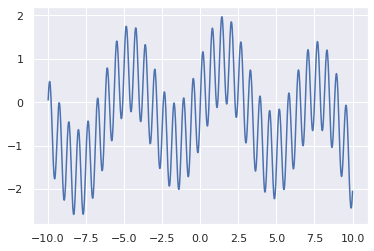
\includegraphics[width=0.8\linewidth]{images/neuropt1.png}
    \caption{png}
\end{figure}

    


The goal is to find $ \arg\max_x O(x) $

\subsection{Evolutionary approach}

Start with an intitial population of 2 instances of $ x $

At every iteration of the evolutionary algorithm, draw $ x_1 $ and $ x_2 $ from the exponential reward distribution:

\begin{equation}
p(x) \sim e^{O(x)}
\end{equation}

And add $ \frac{x_1 + x_2}{2} $ to the population

Repeat for 10000 iterations


From the resulting population of 10002 pick $ x $ with the maximal $ O(x) $



By generating new solutions as modifications of existing successful solutions we focus the search on the most promising part of the search space. The visualization below shows the history of the search, note that the darker colored points were added to the population after the light colored ones. The cross denotes the final solution.


    
\begin{figure}
    \centering
    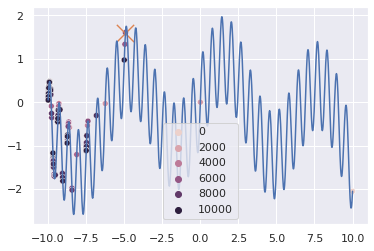
\includegraphics[width=0.8\linewidth]{images/neuropt2.png}
    \caption{png}
\end{figure}

One can see that 10000 iterations were not enough to find the highest peak, although the one we finally found is close. Most of the iterations were spent navigating the far left part of the search space. The right half of the search space remained unexplored - the rightmost solution $ x_\text{right} $ has an $ O(x_\text{right})=-2 $ which means it's almost never drawn from $ p(x) $. This could be mitigated by a number of tricks, for instance, adding a temperature parameter to $ p(x) $:

\begin{equation}
p_t(x) \sim e^{tO(x)}
\end{equation}

but the issue is fundamental to evolutionary algorithms - a few unrepresentative examples can erroneously exclude a large part of the search space.

\subsection{Neural Actor-Critic approach}

In the deep learning approach we train a \emph{critic} neural network $ \hat{O}_{\phi}(x) $ to mimic $ O(x) $ as closely as possible. Then all we need is a second neural network that represents a probability distribution of $ x $s that have a high $ O(x) $ and sample from it. It is called the \emph{actor} network, $ x_{\phi}(z) $, representing a mapping from the normal distribution to the distribution of points with high $ O(x) $. See actor-critic methods\footnote{\url{http://incompleteideas.net/book/first/ebook/node66.html}} in Reinforcement Learning.

We start with an empty population

At every step, we sample $ z $ from $ N(0,1) $, add $ x_{\phi}(z) $ to the population and update both $ \hat{O}_{\phi}(x) $ and $ x_{\phi}(z) $.


    
\begin{figure}
    \centering
    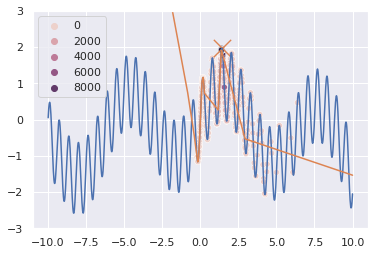
\includegraphics[width=0.8\linewidth]{images/neuropt3.png}
    \caption{png}
\end{figure}

    


\subsection{Neurogenetic approach}

    
\begin{figure}
    \centering
    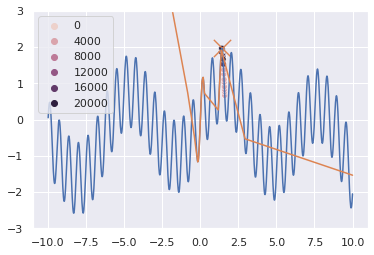
\includegraphics[width=0.8\linewidth]{images/neuropt4.png}
    \caption{png}
\end{figure}

    

One can see that in the hybrid neural-genetic mode, the search process zeros in on the maximum really fast and finds it within 4000 iterations, faster than both pure neural and pure genetic approaches 

\subsection{Going beyond this simple example}

A simple $ O(x):R \rightarrow R $ was used to make the illustration as clear and simple as possible. The principle can be applied to any gradient-free optimization task, including complex search spaces where the domain of $ O(x) $ is images, texts or, say, trading strategies. See this paper by a truly brilliant group of authors applying it to the task of program synthesis\footnote{\url{https://arxiv.org/pdf/2102.04231.pdf}}